\subsection{Semi-leptonic Backgrounds}
\label{subsec:SemilepBkg}

The background containing one real muon and one fake muon originates from few-body semi-leptonic \B-decays.
When the neutrino from such decay carries a low momentum, signal $B$-candidates can be formed with invariant masses falling into the mass window cuts, though are typically at lower mass values, i.e. in the lower mass sideband. 
The main contributions to this background are the \BdPiMuNu and the \BsKMuNu decays. 
Also contributing to this background are the \LPMuNu (and its charge conjugate \AntiLPMuNu) decays, for which the mass distribution extends closer to the signal region. 
The total size of the one fake one real muon background entering into the SR is small such that in the baseline signal channel fit it is absorbed into other components, and the lack of explicit modelling of this background is treated as a systematic uncertainty. 
To assess this uncertainty, what is needed is an estimate of the total size of the one fake and one muon background in the SR and its functional from, the latter being assessed using a merged MC sample.  
These aspects are explained in the following subsections. 

\subsubsection{Normalisation}
\label{subsec:SemiLepNormalisation}

An estimate for the total amount of the one real one fake muon background in each of the BDT output score bins is computed by solving a set of simultaneous equations based upon the data counts in the low mass side band for different muon WPs and the ratio of tight to loose muon efficiencies for both real and fake muons.  
Explicitly, requiring the two muons to pass only the loose WP, the data count in the lower mass side band can be written as 
\begin{equation}
  N_{LL} = N^{\text{ReRe}}_{LL} + N^{\text{ReF}}_{LL} + N^{\text{FF}}_{LL},
  \label{eq:SemiLepLL}
\end{equation}
in which $N^{\text{ReRe}}_{LL}$ is the total amount of candidates in the Loose-Loose (LL) region formed of two Real ($\text{Re}$) muons, $N^{\text{ReF}}_{LL}$ is the number of candidates with one real and one fake (F) muons and $N^{\text{FF}}_{LL}$ is the number of candidates with two fake muons (expected to be very small). 
Similar equations can be written for the requiring only one of the muons to be tight or both of the muons to be tight, 
\begin{equation}
  N_{TL} = N^{\text{ReRe}}_{TL} + N^{\text{ReF}}_{TL} + N^{\text{FF}}_{TL},
  \label{eq:SemiLepTL}
\end{equation}
\begin{equation}
  N_{TT} = N^{\text{ReRe}}_{TT} + N^{\text{ReF}}_{TT} + N^{\text{FF}}_{TT}.
  \label{eq:SemiLepTT}
\end{equation}
Each of the components in the different regions can be related using the fake rates via,
\begin{equation}
  N^\text{ReRe}_{TT} = N^\text{ReRe}_{LL} (\epsilon^{\text{Re}}_{T}/\epsilon^{\text{Re}}_{L})^{2},  \\
\end{equation}
\begin{equation}
  N^\text{ReF}_{TT} = N^\text{ReF}_{LL} (\epsilon^{\text{Re}}_{T}/\epsilon^{\text{Re}}_{L}) (\epsilon^{\text{F}}_{T}/\epsilon^{\text{F}}_{L}), \\ 
\end{equation}
\begin{equation}
  N^\text{FF}_{TT} = N^\text{FF}_{LL} (\epsilon^{\text{F}}_{T}/\epsilon^{\text{F}}_{L})^{2},  
\end{equation}
where $\epsilon^{\text{Re}}_{T}$ is for example the tight WP efficiency for a real muon. 
Similarly, for the LT region
\begin{equation}
  N^\text{ReRe}_{LT} = N^\text{ReRe}_{LL} (1-(\epsilon^{\text{Re}}_{LNT}/\epsilon^{\text{Re}}_{L})^{2}),
\end{equation}
\begin{equation}
  N^\text{ReF}_{LT} = N^\text{ReF}_{LL} (1-(\epsilon^{\text{Re}}_{LNT}/\epsilon^{\text{Re}}_{L}) (\epsilon^{\text{F}}_{LNT}/\epsilon^{\text{F}}_{L})),  
\end{equation}
\begin{equation}
  N^\text{FF}_{LT} = N^\text{FF}_{LL} (1-(\epsilon^{\text{F}}_{LNT}/\epsilon^{\text{F}}_{L})^{2},
\end{equation}
where for convenience the efficiencies for Loose-Not-Tight (LNT) selections are introduced. 
Substituting these into equations~\ref{eq:SemiLepTL} and~\ref{eq:SemiLepTT} yields three equations with three unknowns which can be solved. 
Further, noting that $\epsilon_{LNT} = \epsilon_{L} - \epsilon_{T}$, it can be seen the solution depends only on the ratio of $\epsilon_{T}/\epsilon_{L}$ for real and fake muons, not the absolute fake rates. 
For real muons, this ratio is $\epsilon^{\text{Re}}_{T}/\epsilon^{\text{Re}}_{L} = (0.899 \pm 0.001) /(0.997 \pm 0.001) = 0.9017 \pm 0.0014$ where the uncertainty conservatively assumes the uncertainties on the individual efficiencies are uncorrelated.   

For fake muons, the ratio is taken based upon the \Bhh MC yields in the previous subsection, which yields a value of $\epsilon^{\text{F}}_{T}/\epsilon^{\text{F}}_{L} = 0.45 \pm 0.04$. 
As an alternative, the fake rates computed in sections~\ref{subsubsec:estimation-of-K-to-ell} and~\ref{subsubsec:estimation-of-Pi-to-ell} could be used, however using the \Bhh MC fake rates has the advantage of being in the SR phase space. 
Additionally, this value for the ratio is higher than using the fake rates in the previous section, making this choice the more conservative approach. 

Using these ratios and the data counts, the yields in Table~\ref{tab:SemiLepYields} are obtained.  
From this it can be seen that the fraction of semi-leptonic events in the sideband ranges from 3\% - 37\% across the BDT bins, with a higher fraction in the more signal like bins.  
These yields are used to normalise the merged semi-leptonic MC sample discussed in the next section. 
\begin{table}[h]
  \centering
  \begin{tabular}{ccccc}
    \toprule
    BDT bin & $N^{\text{ReRe}}$ & $N^{\text{ReF}}$ & $N^{\text{FF}}$ & $N^{\text{Total}}$ \\ 
    \midrule
    0 & 9970 ± 89 & 333 ± 41 & 11.7 ± 2.5 & 10314 \\
    1 & 1406 ± 30 & 146 ± 12 & 7.0 ± 1.5 & 1559 \\
    2 & 398 ± 15 & 74.4 ± 6.1 & 3.12 ± 0.65 & 476 \\
    3 & 99 ± 11 & 56.8 ± 5.8 & -0.43 ± 0.13 & 155 \\ 
    \bottomrule
  \end{tabular}
  \caption{Yields of candidates with two real, one real-one fake, and two fake muons in the low mass sideband in the signal channel for both muon candidates passing the tight WP. }
  \label{tab:SemiLepYields}
\end{table}



\subsubsection{Merged Monte Carlo Sample}
\label{subsec:SemiLepMCmerging}

To evaluate the impact of the semileptonic background, a functional form for this component is derived using MC simulation. 
Separate MC samples are produced for the \BdPiMuNu, \BsKMuNu, \LPMuNu and \AntiLPMuNu decays. 
These samples are then merged together into one semileptonic sample. 
To get the relative normalisation of each of the samples for this merging, the following approach is taken. 
First, the relative production rates of respective baryons are considered, with the \Bs and $\Lambda_{b}$ production fractions being lower than \Bd by the hadronic production fractions $f_{s}/f_{d}$ and $f_{\Lambda_{b}}/f_{d}$ respectively. 
The values used are $f_{s}/f_{d} = 0.256$~\cite{HFLAV:2016hnz} and $f_{\Lambda_{b}}/f_{d} = 0.8$~\cite{LHCb:2011leg}, where in the latter it is taken that $f_{u} = f_{d}$.
The ratio  $f_{\Lambda_{b}}/f_{\bar{\Lambda}_{b}}$ is also taken to be equal to one based upon the studies in Ref.~\cite{CMS:2012wje}.
These values are only approximate, but are considered to be sufficient given the semileptonic background is treated as a systematic. 

Second, the efficiencies of these samples passing the nominal selections is considered. 
Due to the relatively small statistics and low fake rates, it is necessary to compute this efficiency in two stages. 
The first stage is applying all the nominal selections except for the trigger and only requiring one of the muons to pass the ID requirements. 
The second is computing the relative efficiency of requiring both muons to pass the ID requirements to only one of them needing to, but without the any of the other selections applied except for the leading (sub-leading) ID tracks to have $\pT > 6\,\GeV (\pT > 4\,\GeV)$. 
This second factor gives an approximation of the relative muon fake rate for the different hadrons. 
The product of these two factors, combined with the relative production fractions, is used to compute the overall relative composition of the semi leptonic background in the SR. 
The relative fractions, for BDT output $>0.1609$ (i.e. the four BDT output bins merged) are found to be 65\% \BdPiMuNu, 16\% \AntiLPMuNu, 14\% \BsKMuNu and 5\% \LPMuNu.  


\subsubsection{Functional Form}
\label{subsec:SemiLepFunctionalForm}

The functional form used for the semi-leptonic decays is exponential plus a Gaussian tail:
\begin{eqnarray}
  F(x) = f \cdot E(x; \alpha) + (1 - f) \cdot G(x; \mu, \sigma)  
       = f \cdot \text{exp}(\alpha x) + (1 - f) \cdot \frac{1}{\sqrt{2\pi\sigma^2}} \text{exp}\left[-\frac{(x - \mu)^2}{2\sigma^2}\right],
  \label{eq:expGaussTail}
\end{eqnarray}
where $\alpha$ is the exponential constant, $f$ is the fraction of the exponential with respect to the Gaussian, and where $\mu$ and $\sigma$ are respectively the mean and sigma of the Gaussian.

To validate the chosen PDF for the semi-leptonic background we fit the dimuon VTX mass distribution from the merged semi-leptonic MC sample for the three modes with the PDF in equation~\ref{eq:expGaussTail}. 
The ID-based VTX mass is used instead of the MUCALC mass since fake muons frequently fail to produce combined muon tracks which are required in the baseline selection, leading to reduced statistics. 
Applied to the semileptonic MC sample is a loosened selection: all final selections apart from the muon quality requirements and passing the online trigger are applied to the merged MC sample to allow for more statistics. 
Loosening the selections on the semi-leptonic MC to extract the shape parameters for this background is justified because this PDF is only used in evaluation of a systematic, it is not used explicitly in the signal channel fit.

Figure~\ref{fig:semilepMCfitLoose} shows the loosened selection MC fit results with the fitted PDF in all BDT output bins satisfactory reproducing the shape of the MC sample as can be seen from the residual distributions. With enough statistics the fit quality is also satisfactory with $p$-value $>$ 0.05 in each bin of the BDT output. 

\begin{figure}[ht!]
  \centering
  \subfloat[BDT bin 0 fit with BDT boundaries at {[0.1609,0.2636]}.]{
    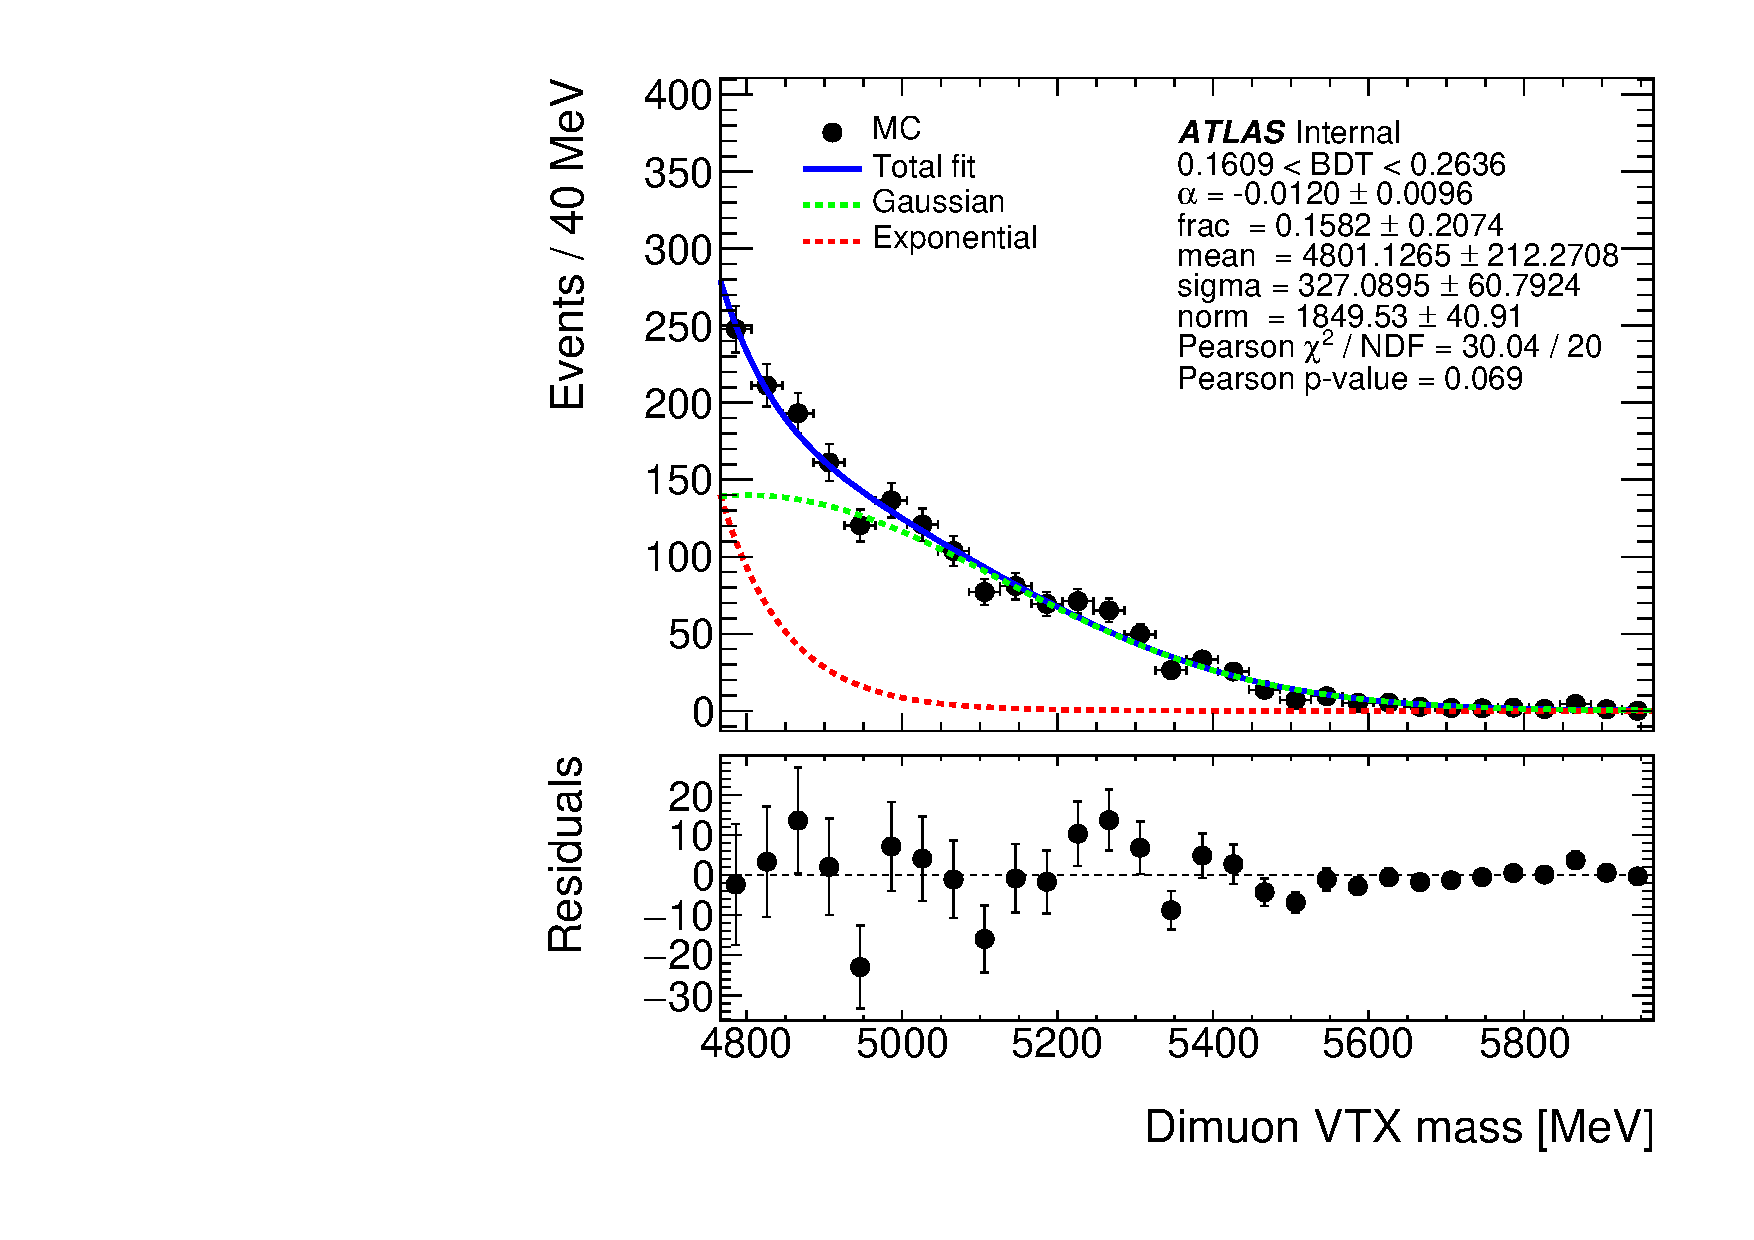
\includegraphics[width=0.5\textwidth]{figures/SignalExtraction/out_fit_test_semilep_v2p4_can_bin_0.pdf}
    \label{fig:semilepMCfitLooseBin0}
  }
  \subfloat[BDT bin 1 fit with BDT boundaries at {[0.2636,0.3405]}.]{
    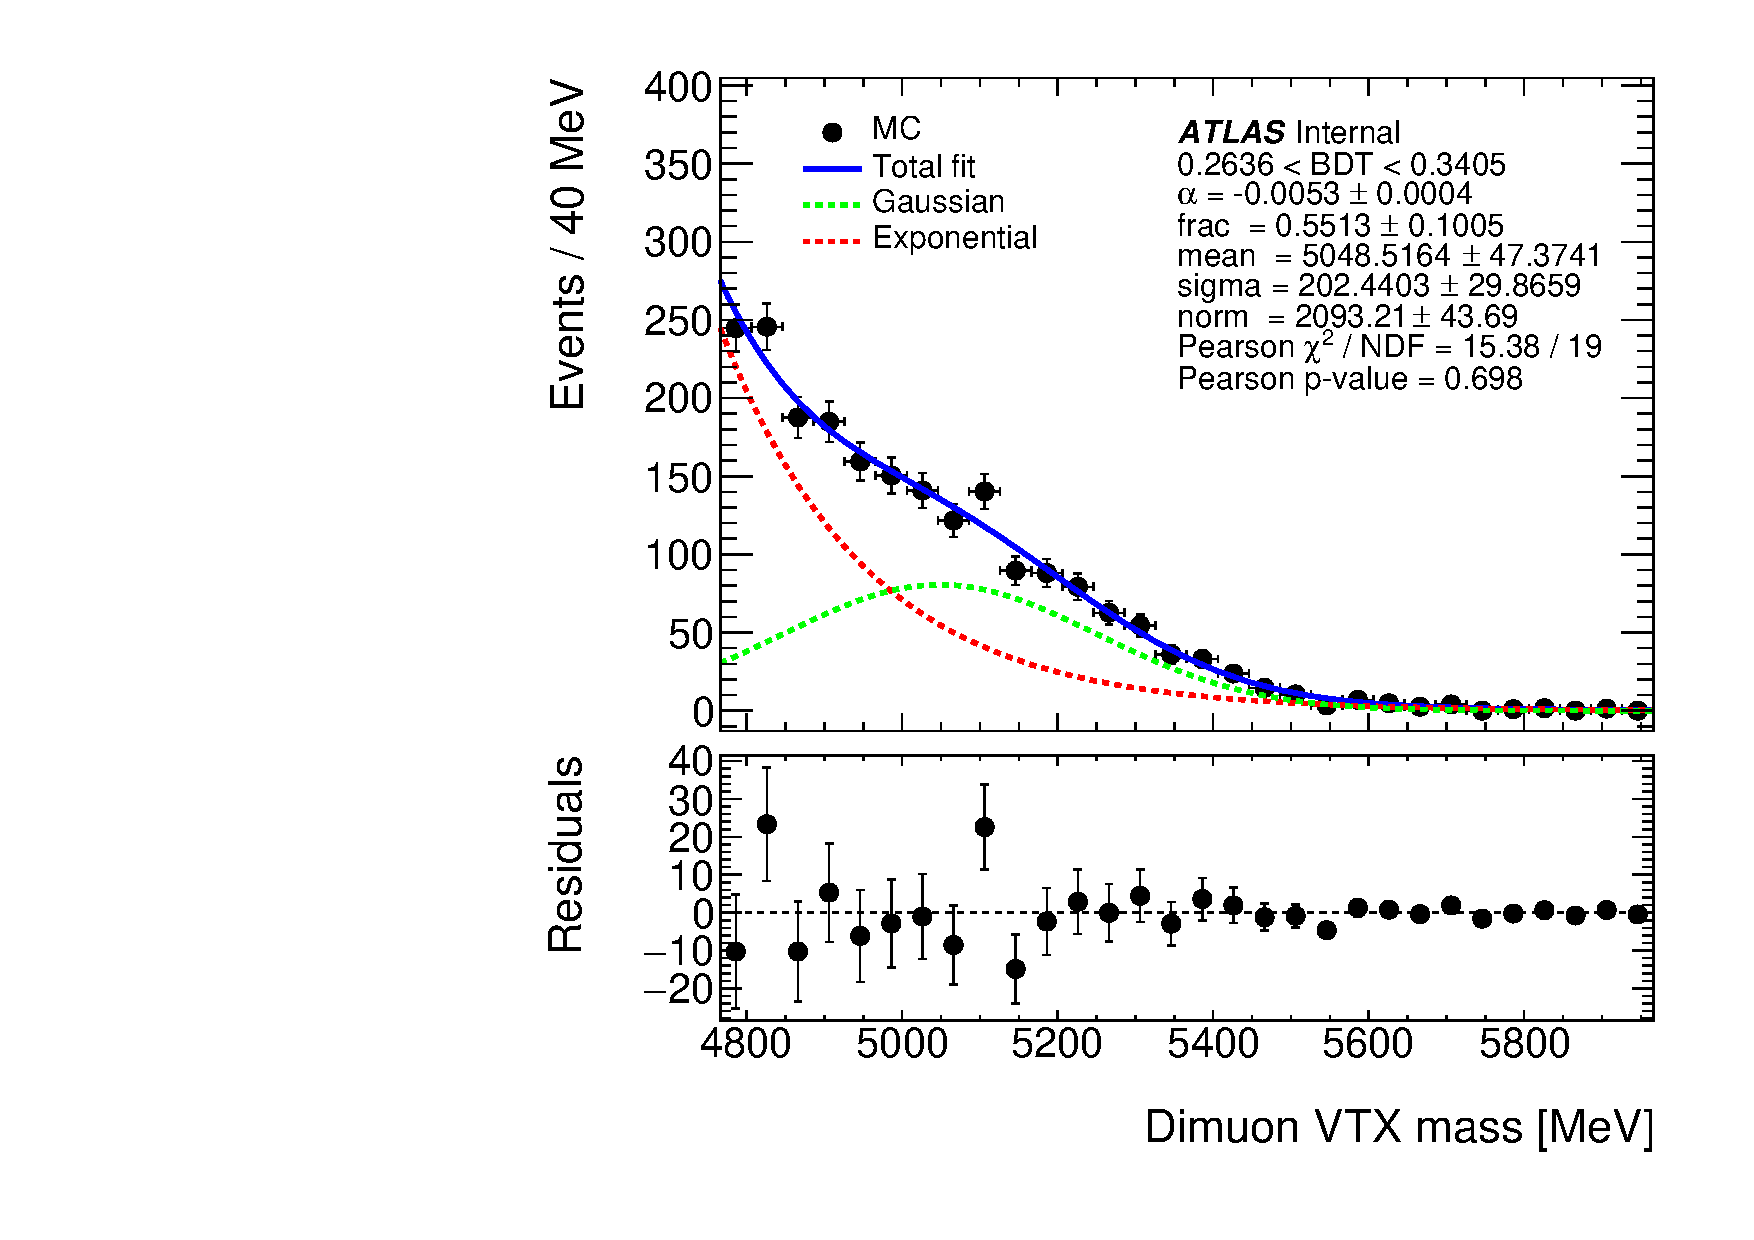
\includegraphics[width=0.5\textwidth]{figures/SignalExtraction/out_fit_test_semilep_v2p4_can_bin_1.pdf}
    \label{fig:semilepMCfitLooseBin1}
  }
  \\
  \subfloat[BDT bin 2 fit with BDT boundaries at {[0.3405,0.4055]}.]{
    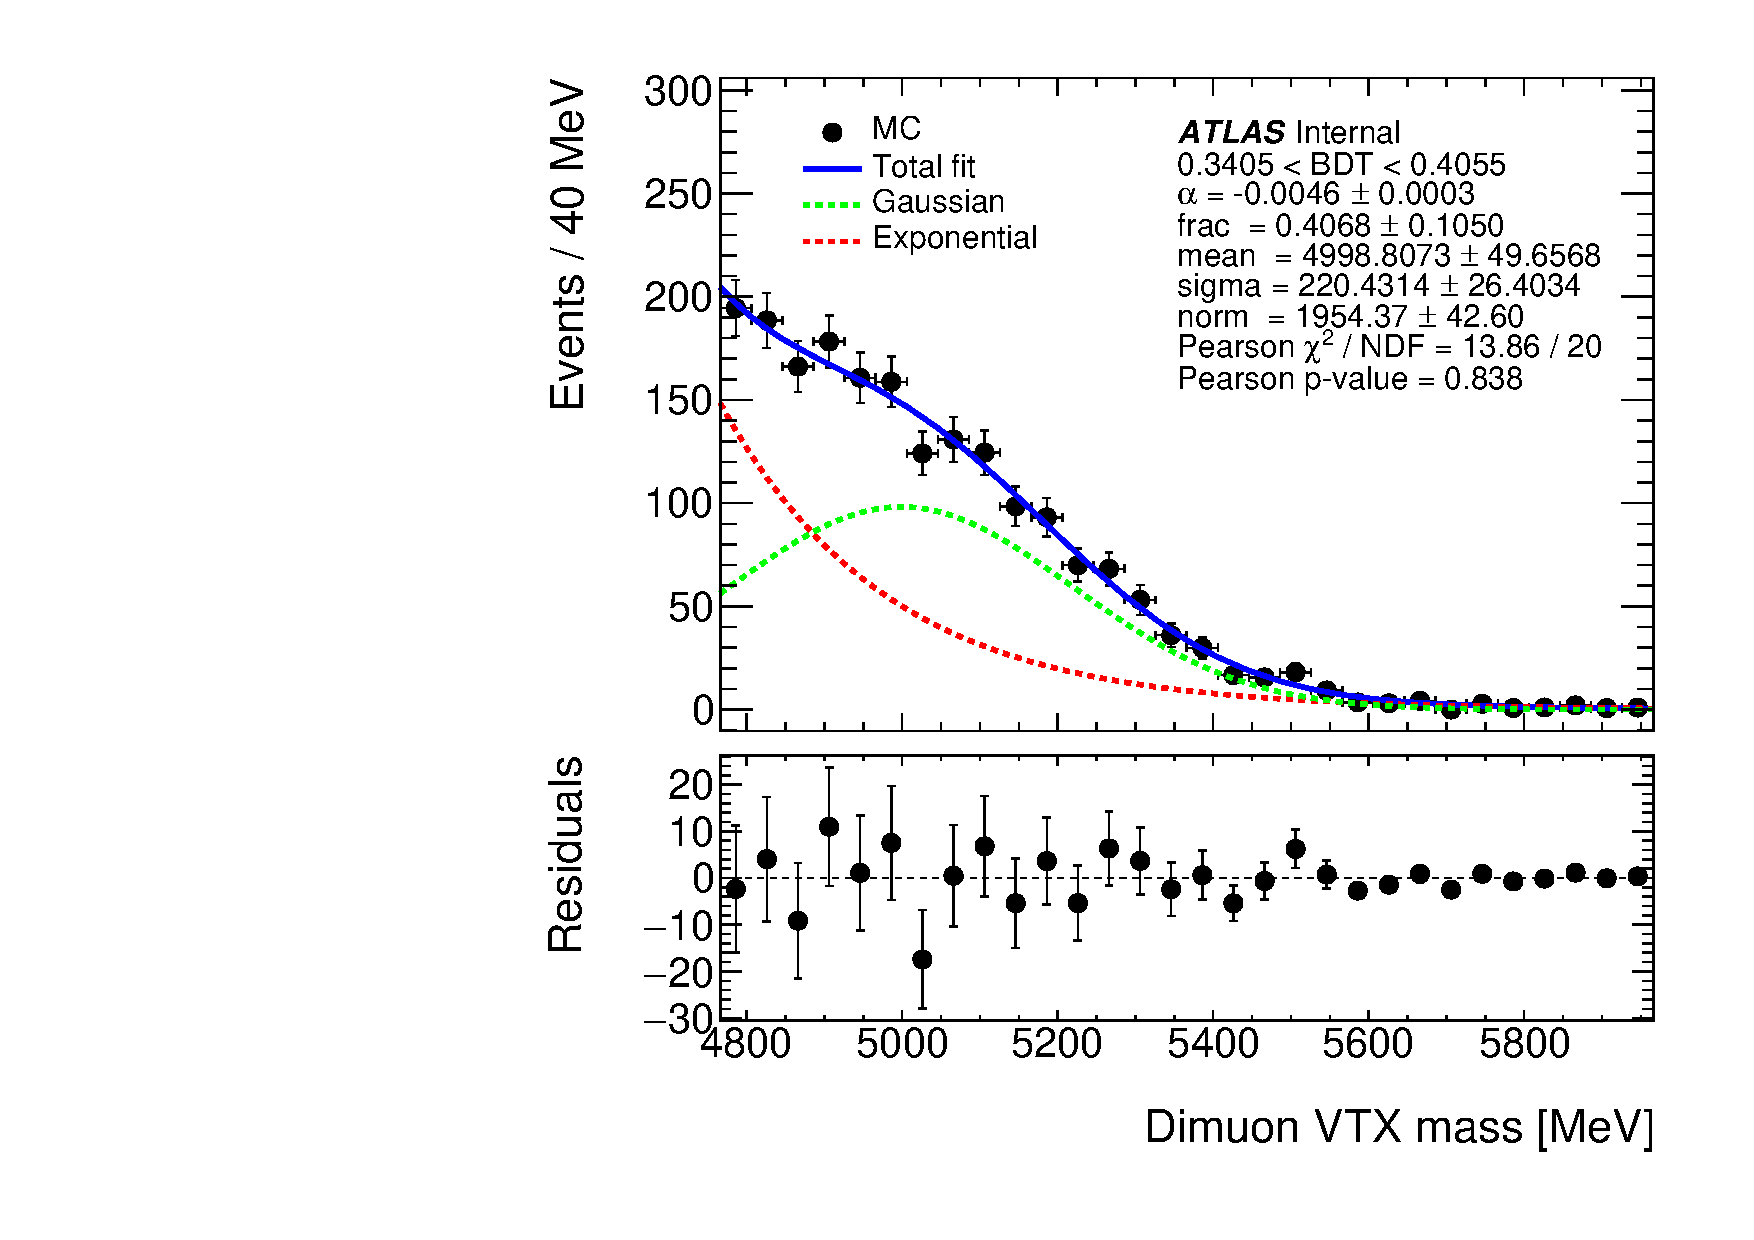
\includegraphics[width=0.5\textwidth]{figures/SignalExtraction/out_fit_test_semilep_v2p4_can_bin_2.pdf}
    \label{fig:semilepMCfitLooseBin2}
  }
  \subfloat[BDT bin 3 fit with BDT boundaries at {[0.4055,1.0000]}.]{
    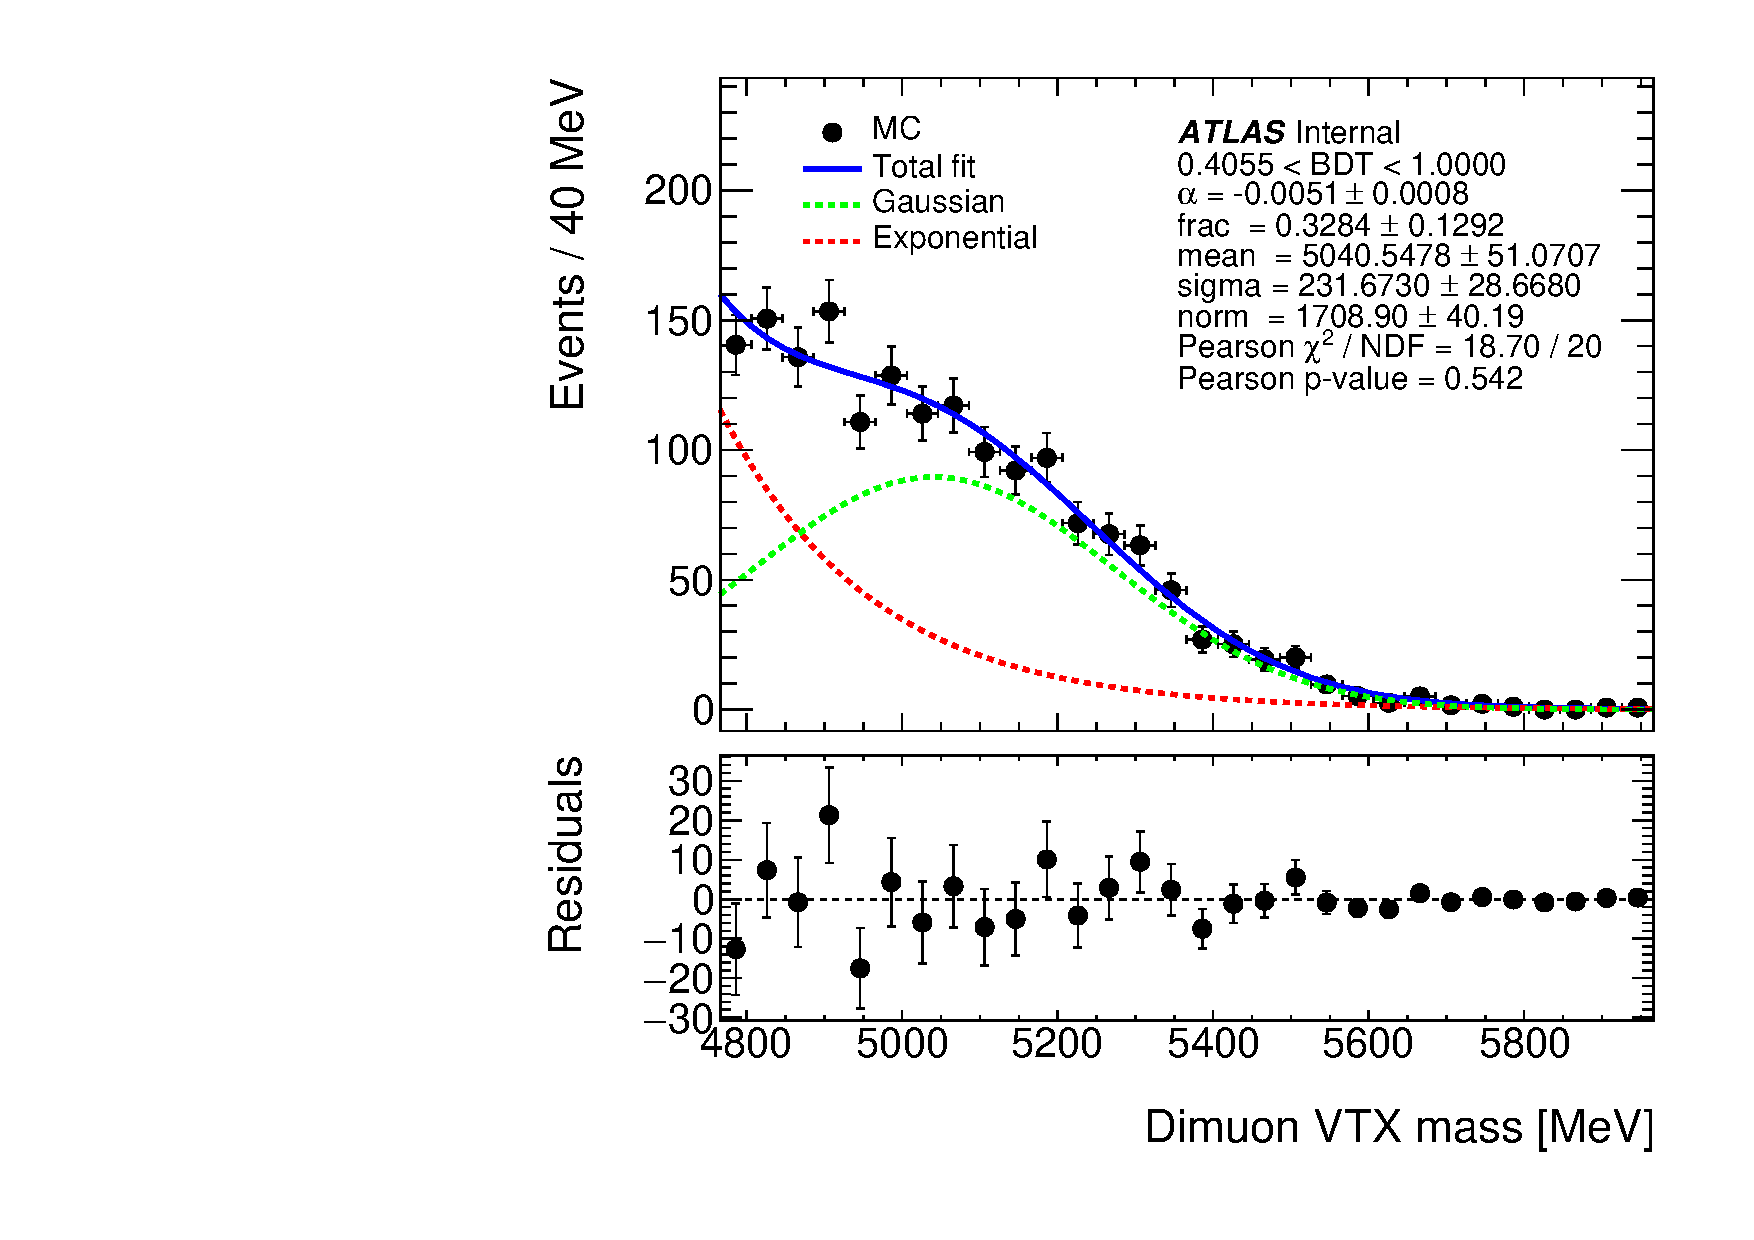
\includegraphics[width=0.5\textwidth]{figures/SignalExtraction/out_fit_test_semilep_v2p4_can_bin_3.pdf}
    \label{fig:semilepMCfitLooseBin3}
  }
  \caption{Unbinned extended maximum likelihood fits performed independently in BDT bin 0 \protect\subref{fig:semilepMCfitLooseBin0}, 1 \protect\subref{fig:semilepMCfitLooseBin1}, 2 \protect\subref{fig:semilepMCfitLooseBin2}, and 3 \protect\subref{fig:semilepMCfitLooseBin3} on the merged \BdPiMuNu, \BsKMuNu, \LPMuNu, and \LPMuNu exclusive MC samples. Applied to the merged MC sample is a loosened selection which comprises of all the final selections except the online trigger (and matching), additionally requiring only one of the offline muons to pass the tight WP and be a combined muon (the other muon is required to only pass the loose WP).} 
  \label{fig:semilepMCfitLoose}
\end{figure}

As a cross-check, these functional forms are checked with the full selection applied with the shape parameters fixed to the results from the fits in the loose regions. 
Figure~\ref{fig:semilepMCfit} shows the results of these fits.
Although the statistics are low, it can be seen the PDFs reproduce satisfactorily the MC shape and with a good fit quality in all bins of the BDT output. 

\begin{figure}[ht!]
  \centering
  \subfloat[BDT bin 0 fit with BDT boundaries at {[0.1609,0.2636]}.]{
    %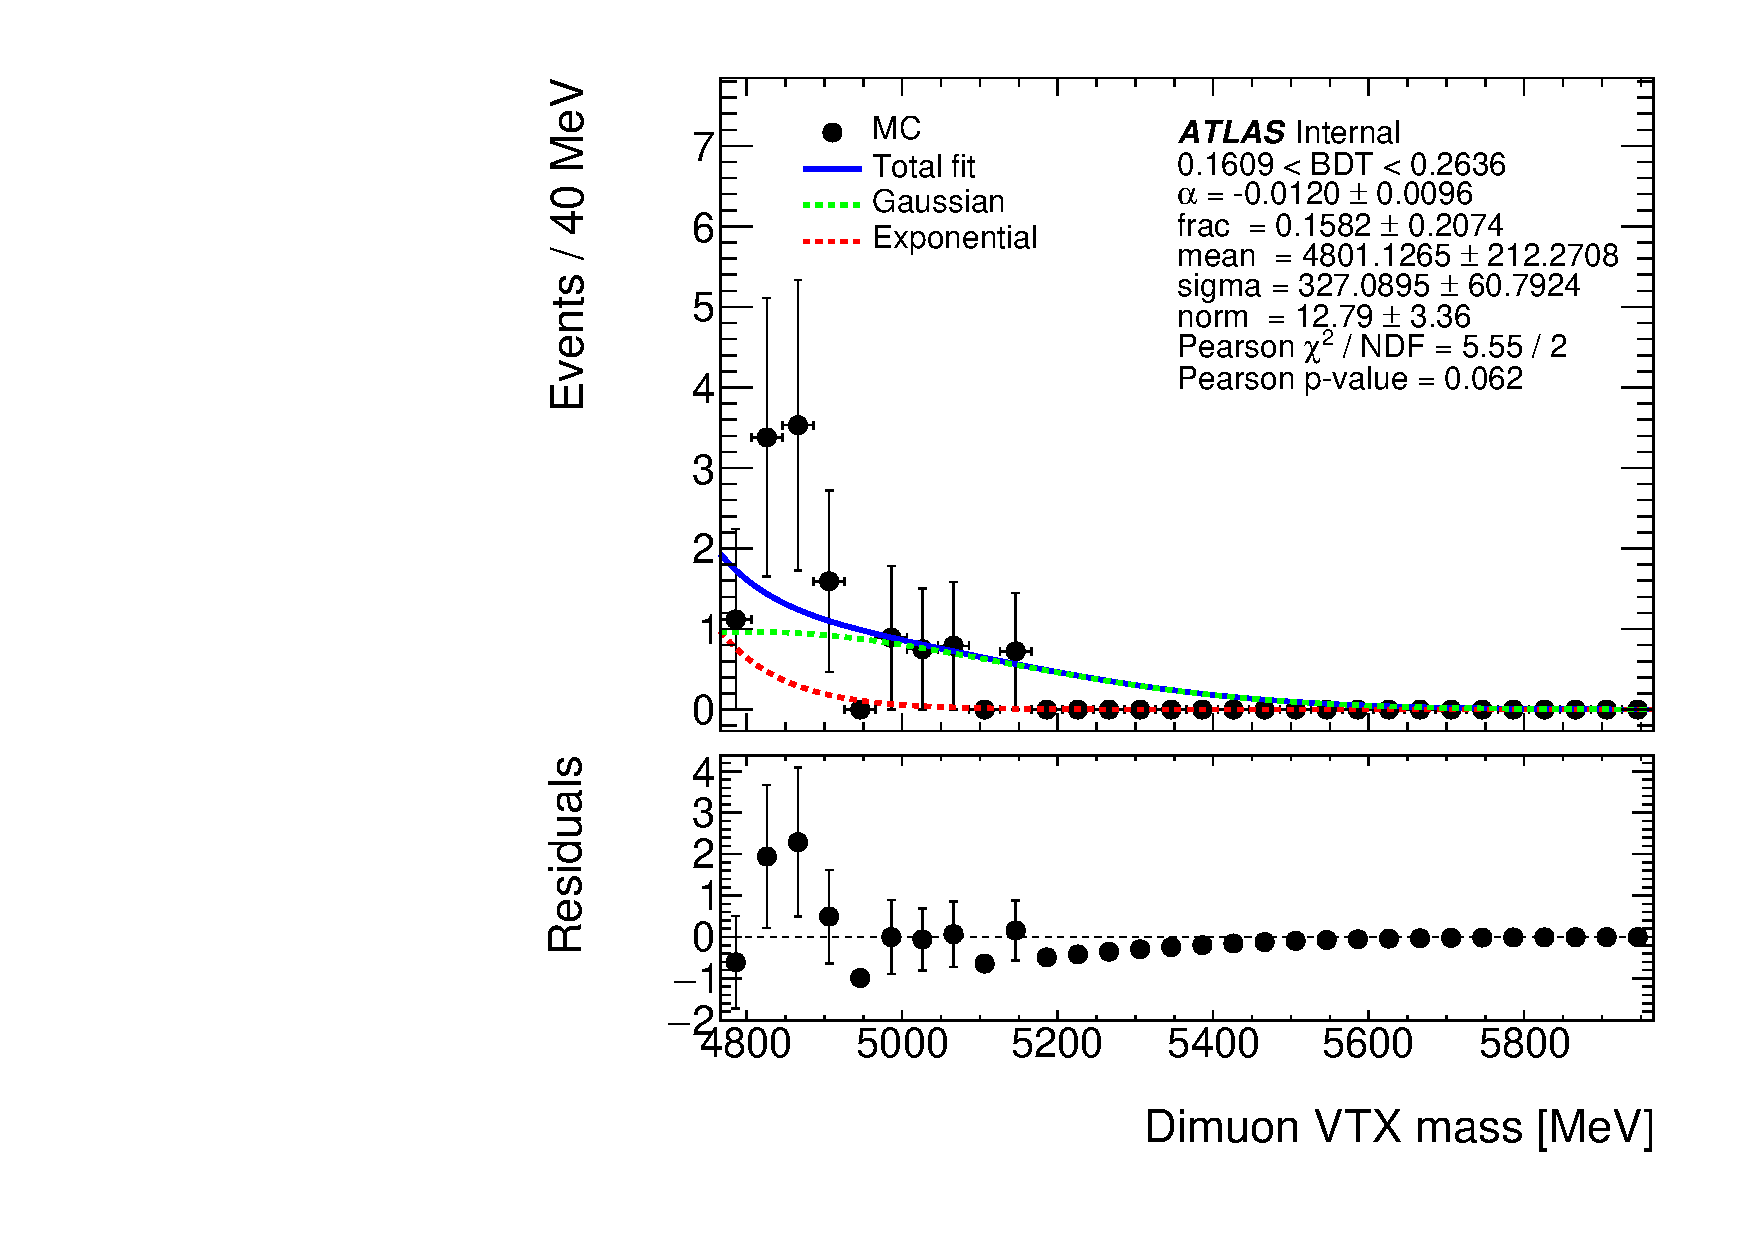
\includegraphics[width=0.5\textwidth]{figures/SignalExtraction/out_fit_test_semilep_v2p4_loose_params_fixed_can_bin_0.pdf} % using Pearson Chi2 and p-value
    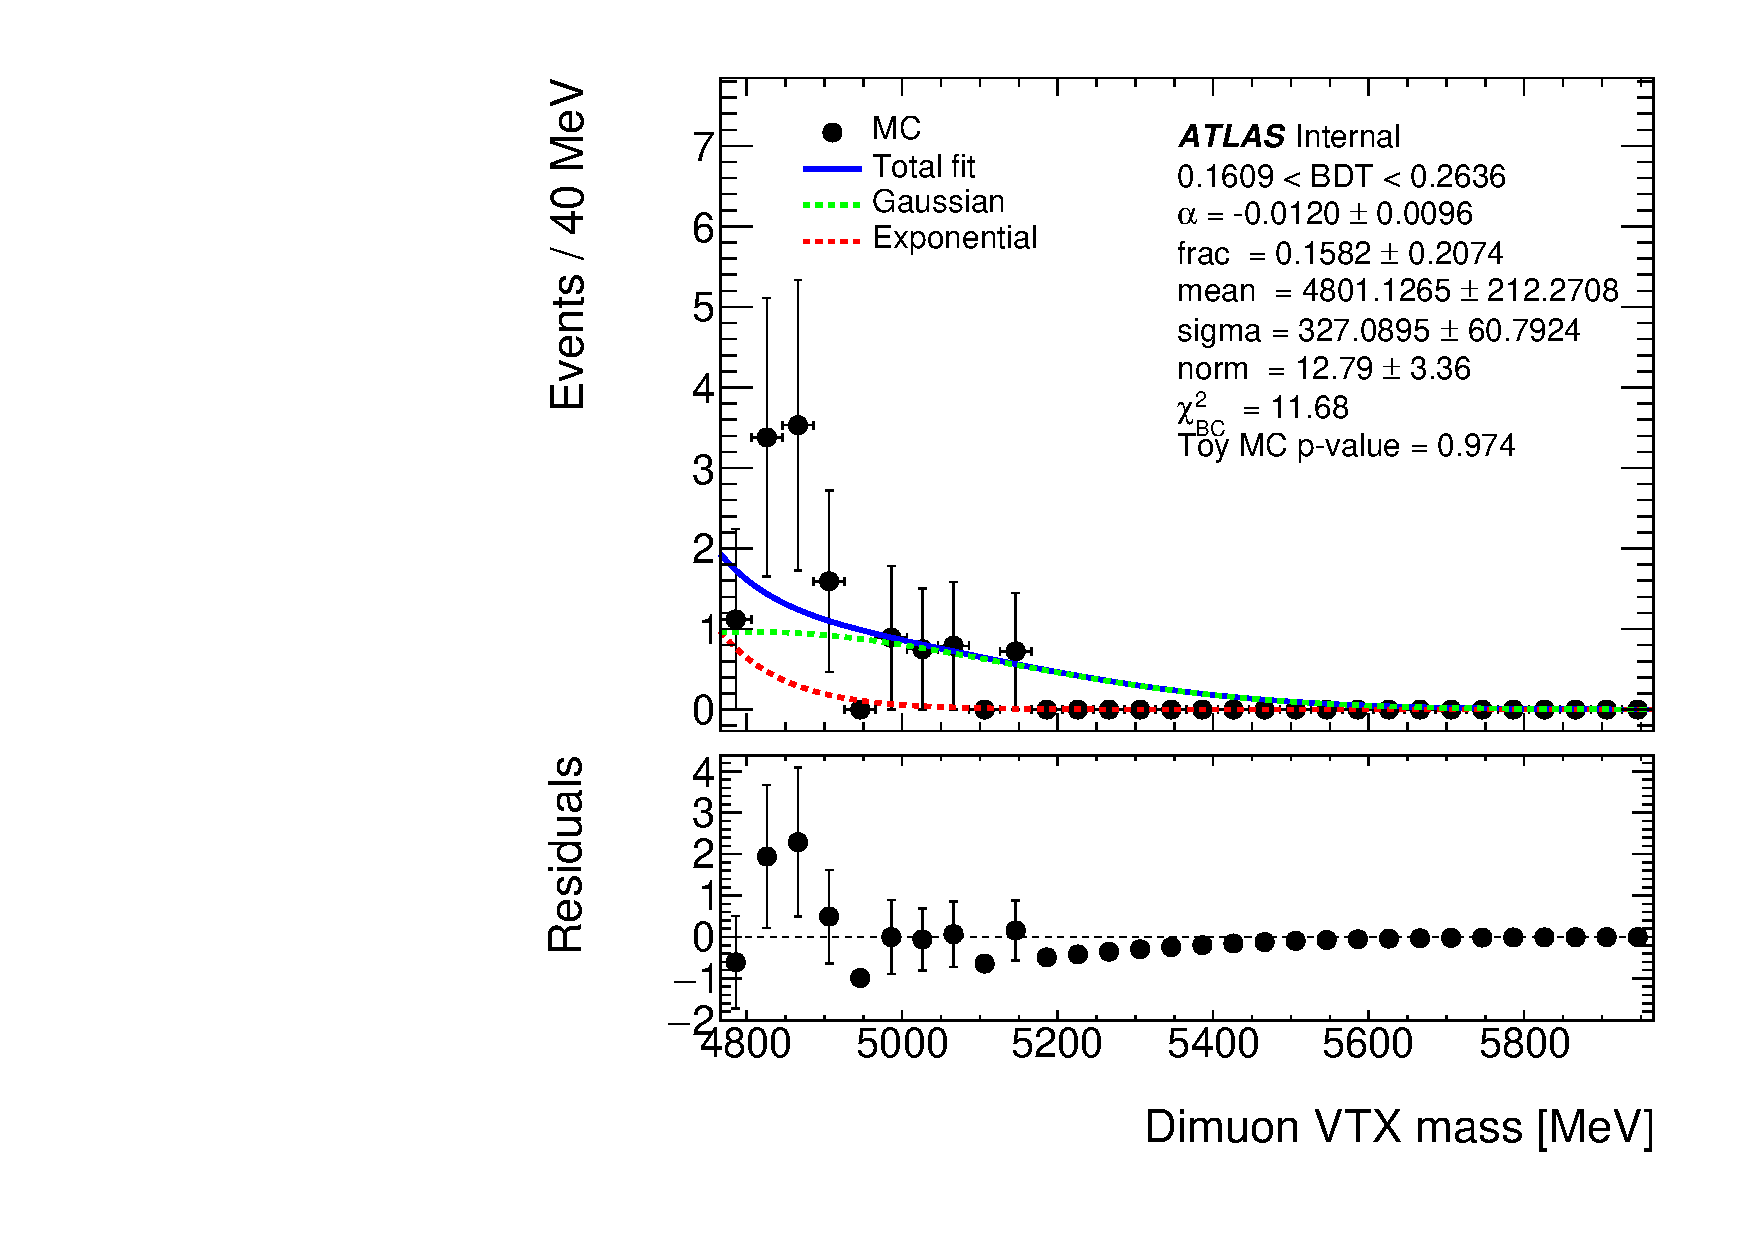
\includegraphics[width=0.5\textwidth]{figures/SignalExtraction/out_fit_semilep_v2p4_loose_params_fixed_BC_toy_MC_p_val_can_bin_0.pdf} % using toy MC BC Chi2 and p-value
    \label{fig:semilepMCfitBin0}
  }
  \subfloat[BDT bin 1 fit with BDT boundaries at {[0.2636,0.3405]}.]{
    %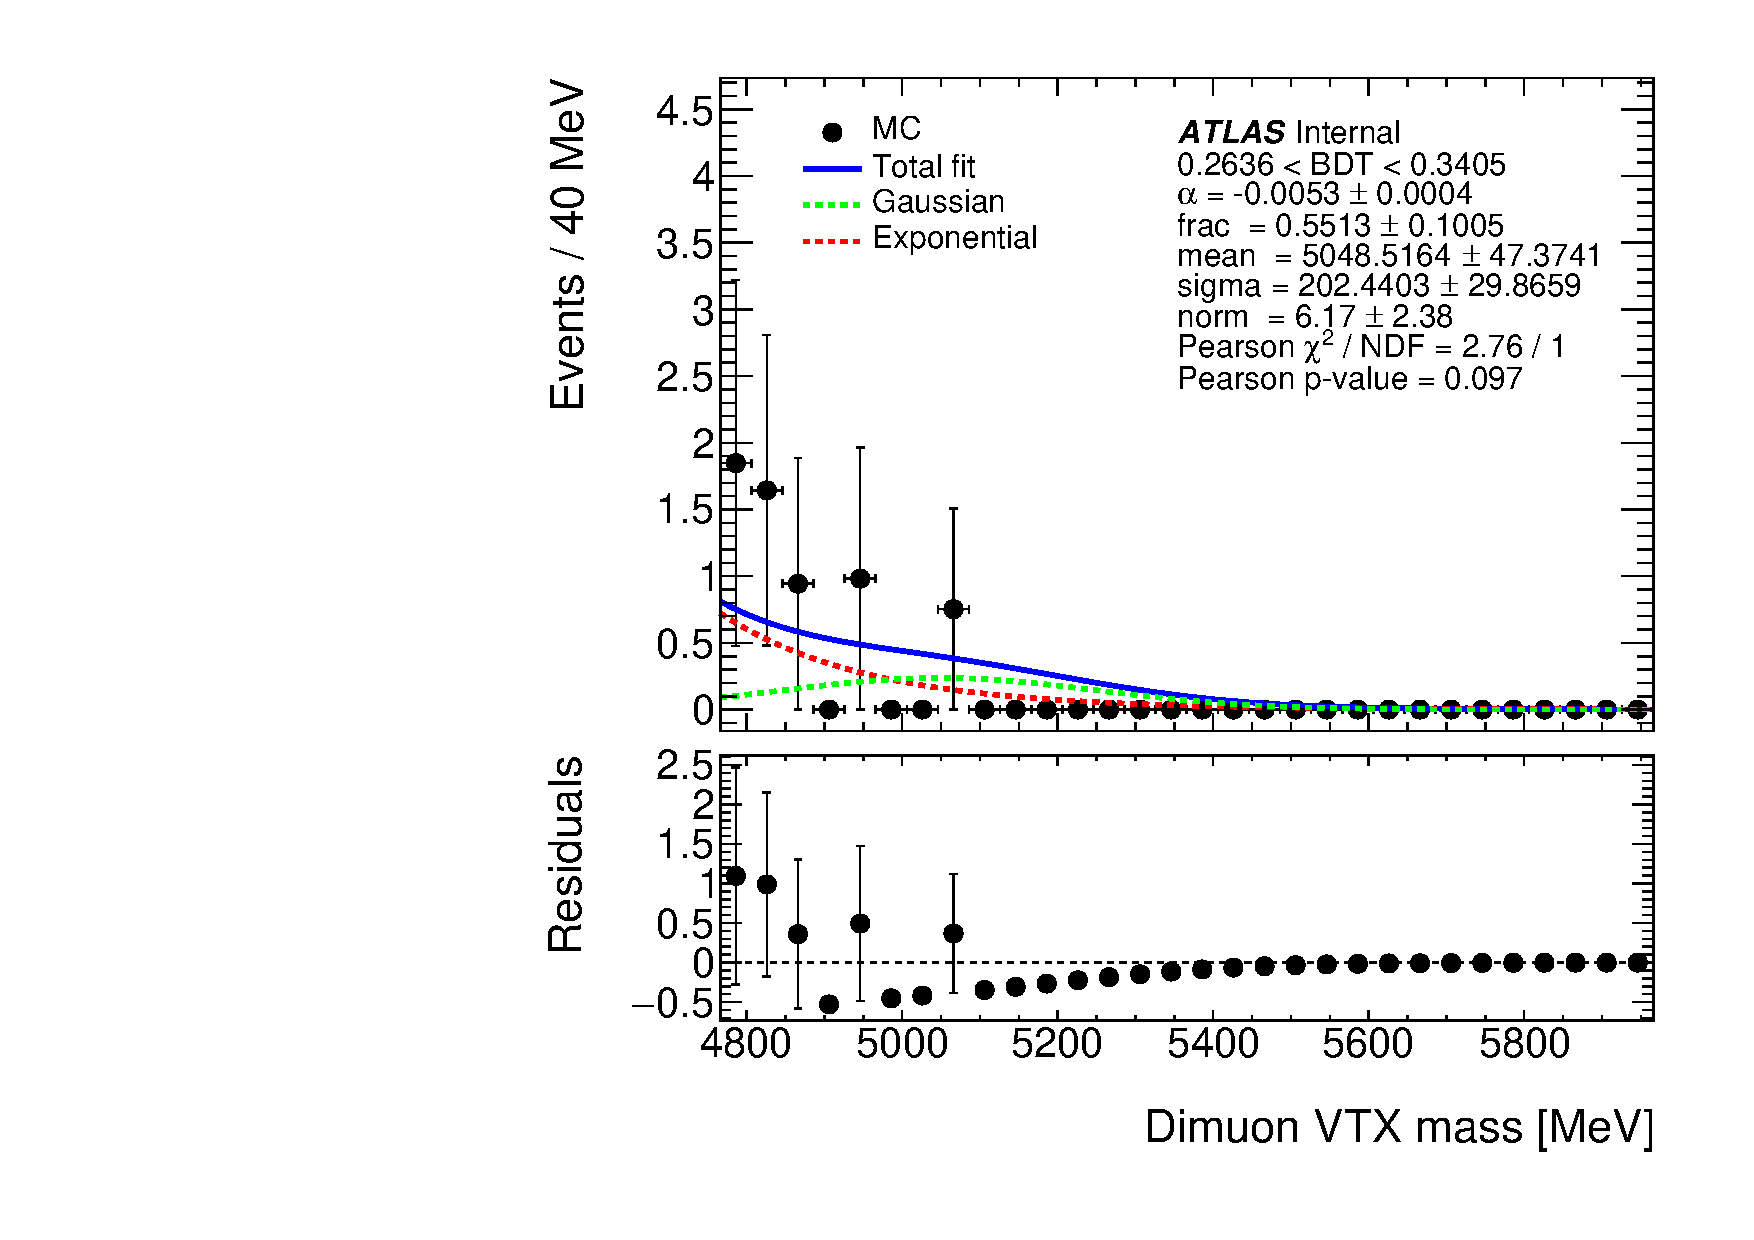
\includegraphics[width=0.5\textwidth]{figures/SignalExtraction/out_fit_test_semilep_v2p4_loose_params_fixed_can_bin_1.pdf}
    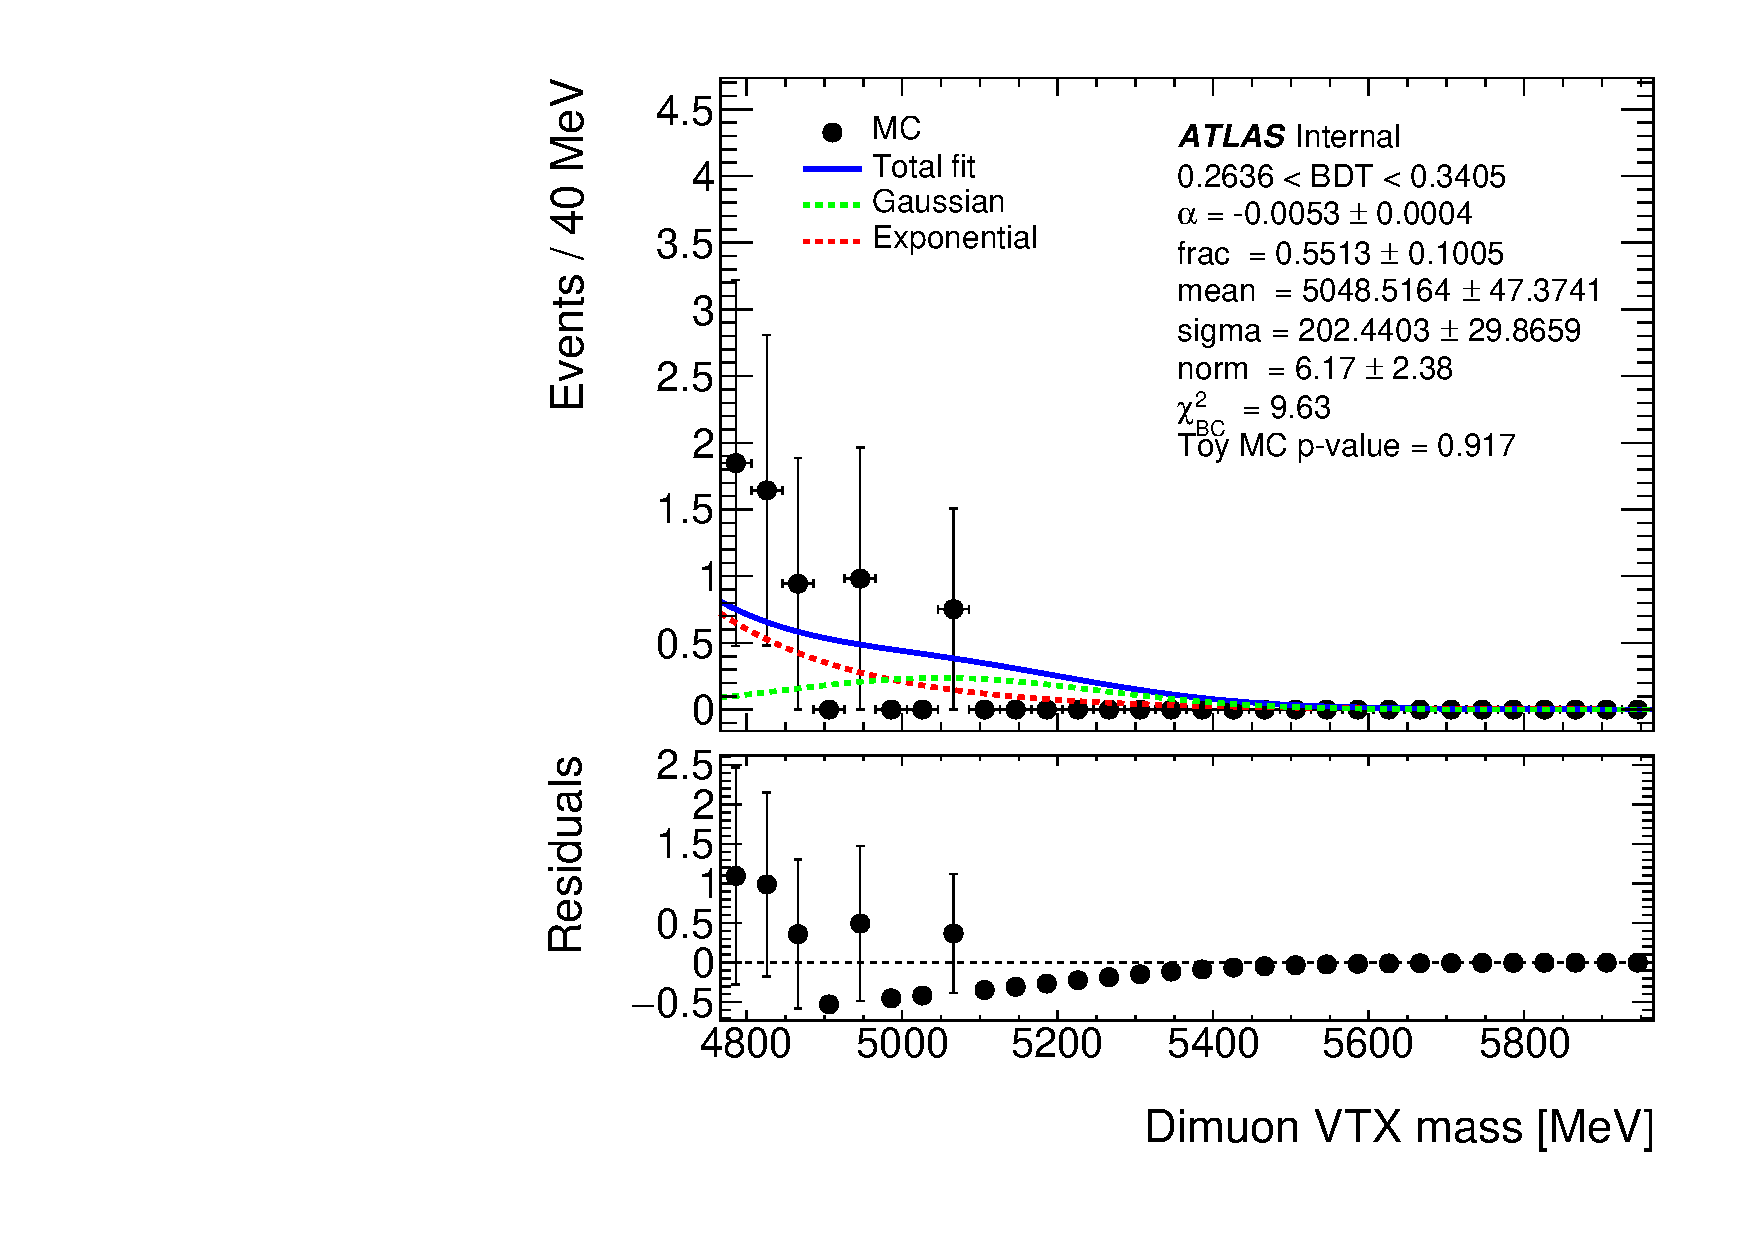
\includegraphics[width=0.5\textwidth]{figures/SignalExtraction/out_fit_semilep_v2p4_loose_params_fixed_BC_toy_MC_p_val_can_bin_1.pdf} % using toy MC BC Chi2 and p-value
    \label{fig:semilepMCfitBin1}
  }
  \\
  \subfloat[BDT bin 2 fit with BDT boundaries at {[0.3405,0.4055]}.]{
    %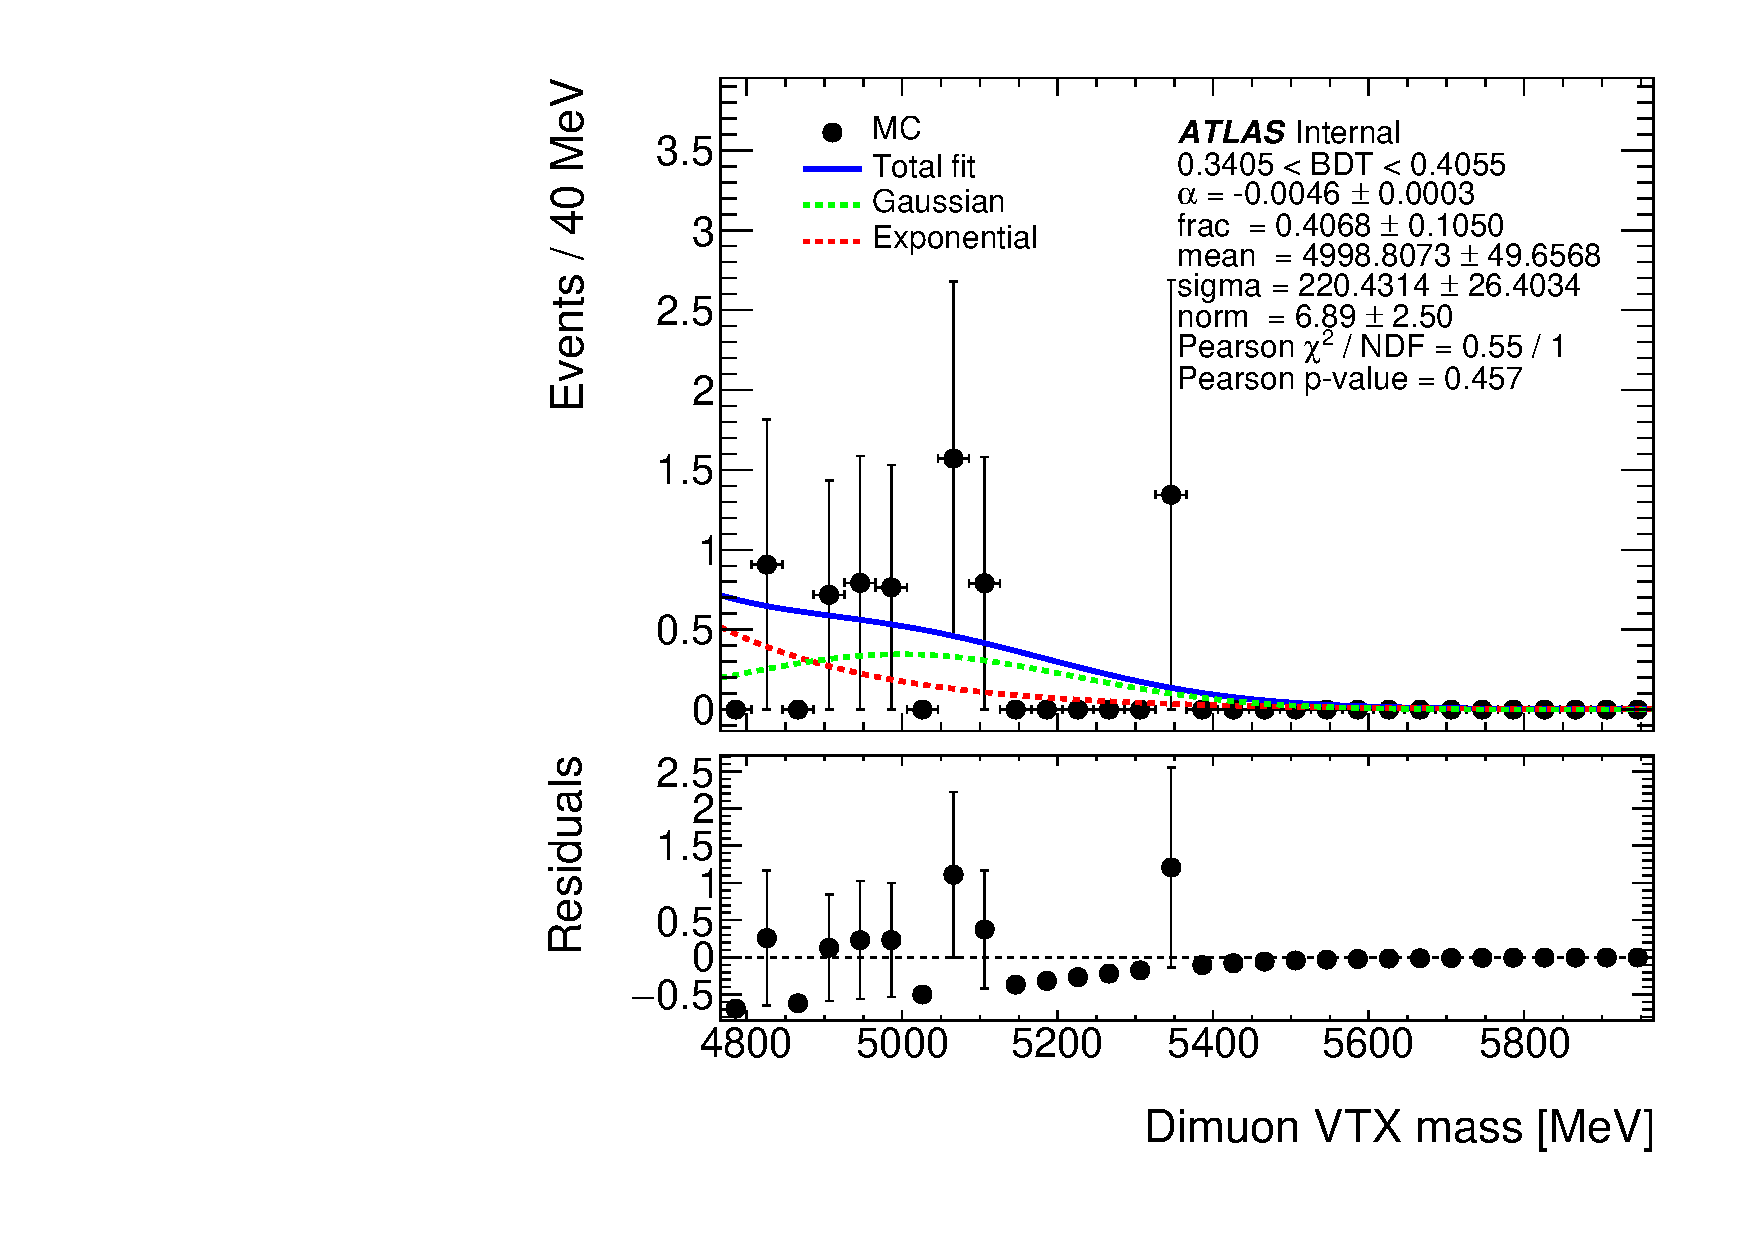
\includegraphics[width=0.5\textwidth]{figures/SignalExtraction/out_fit_test_semilep_v2p4_loose_params_fixed_can_bin_2.pdf}
    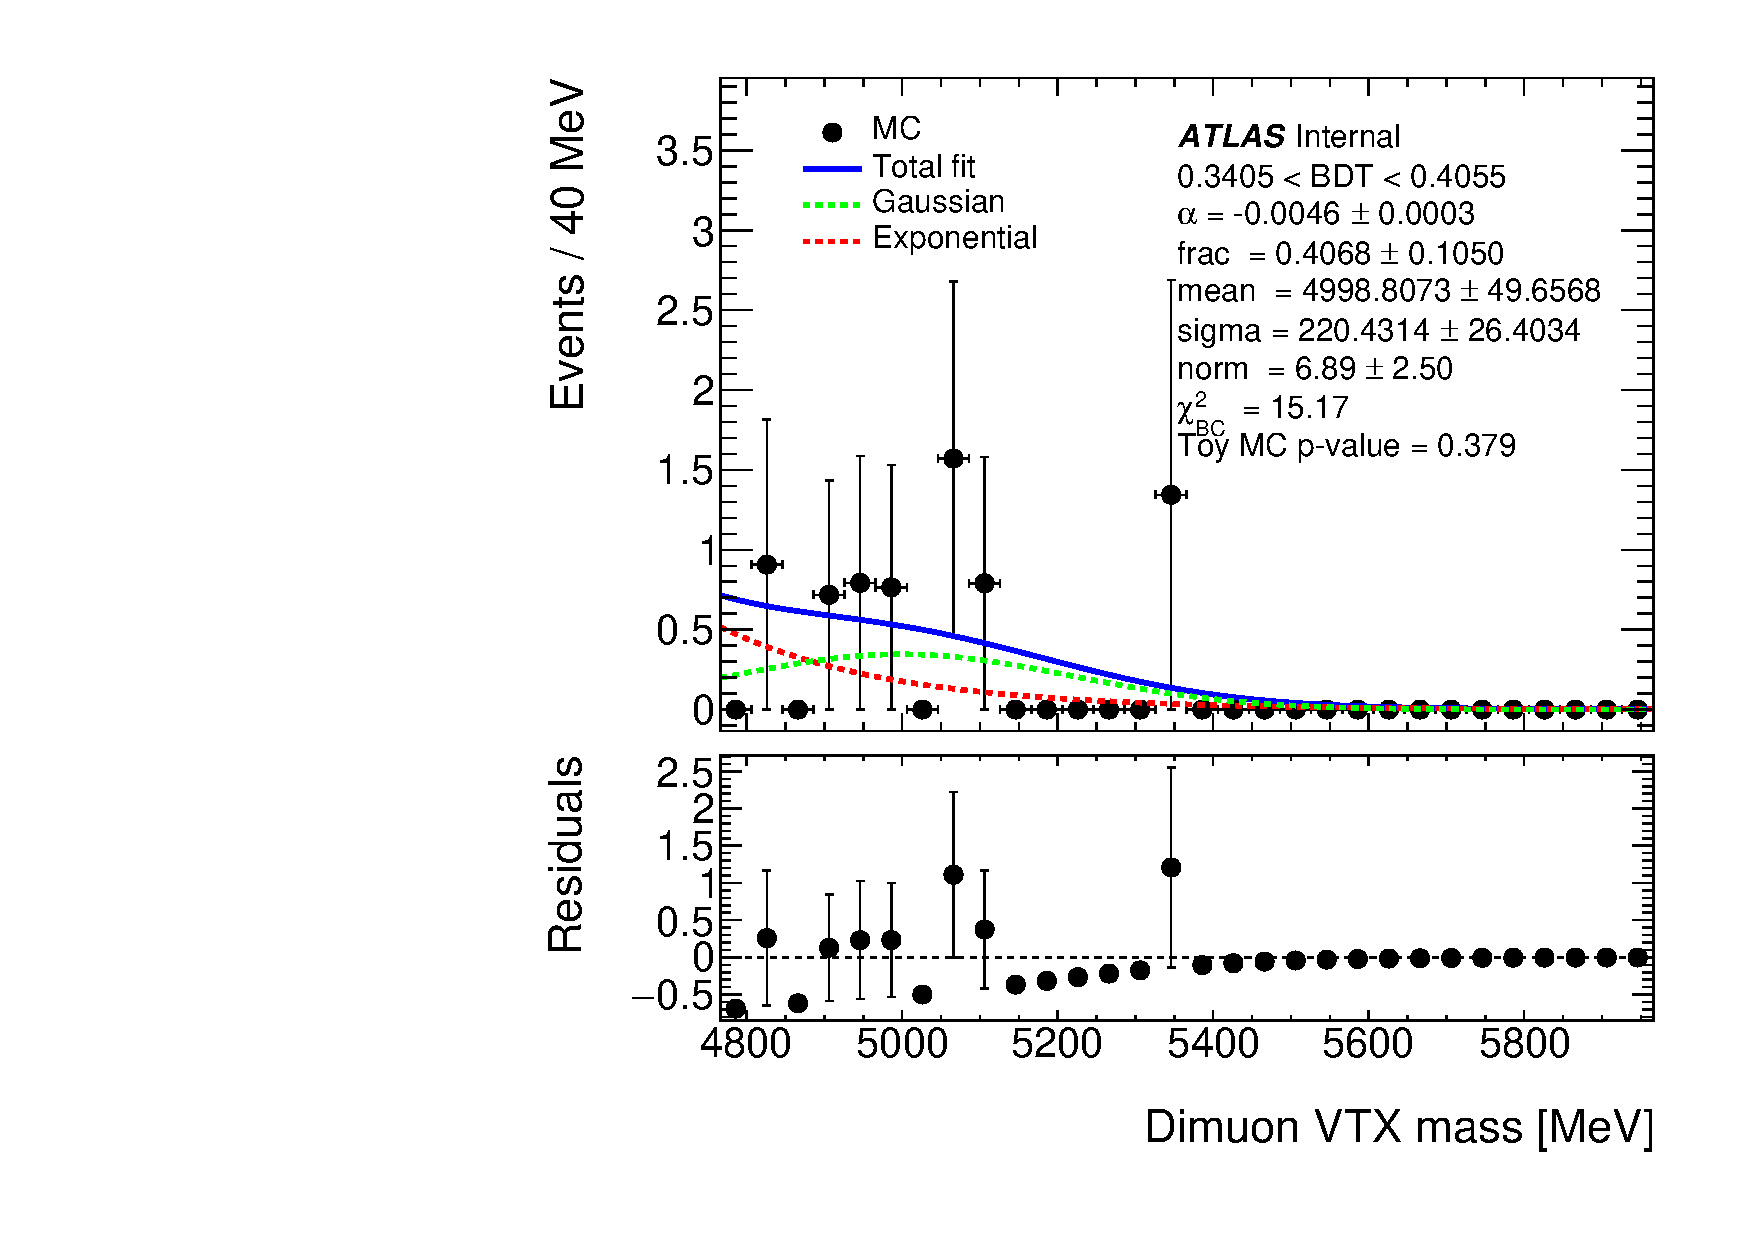
\includegraphics[width=0.5\textwidth]{figures/SignalExtraction/out_fit_semilep_v2p4_loose_params_fixed_BC_toy_MC_p_val_can_bin_2.pdf} % using toy MC BC Chi2 and p-value
    \label{fig:semilepMCfitBin2}
  }
  \subfloat[BDT bin 3 fit with BDT boundaries at {[0.4055,1.0000]}.]{
    %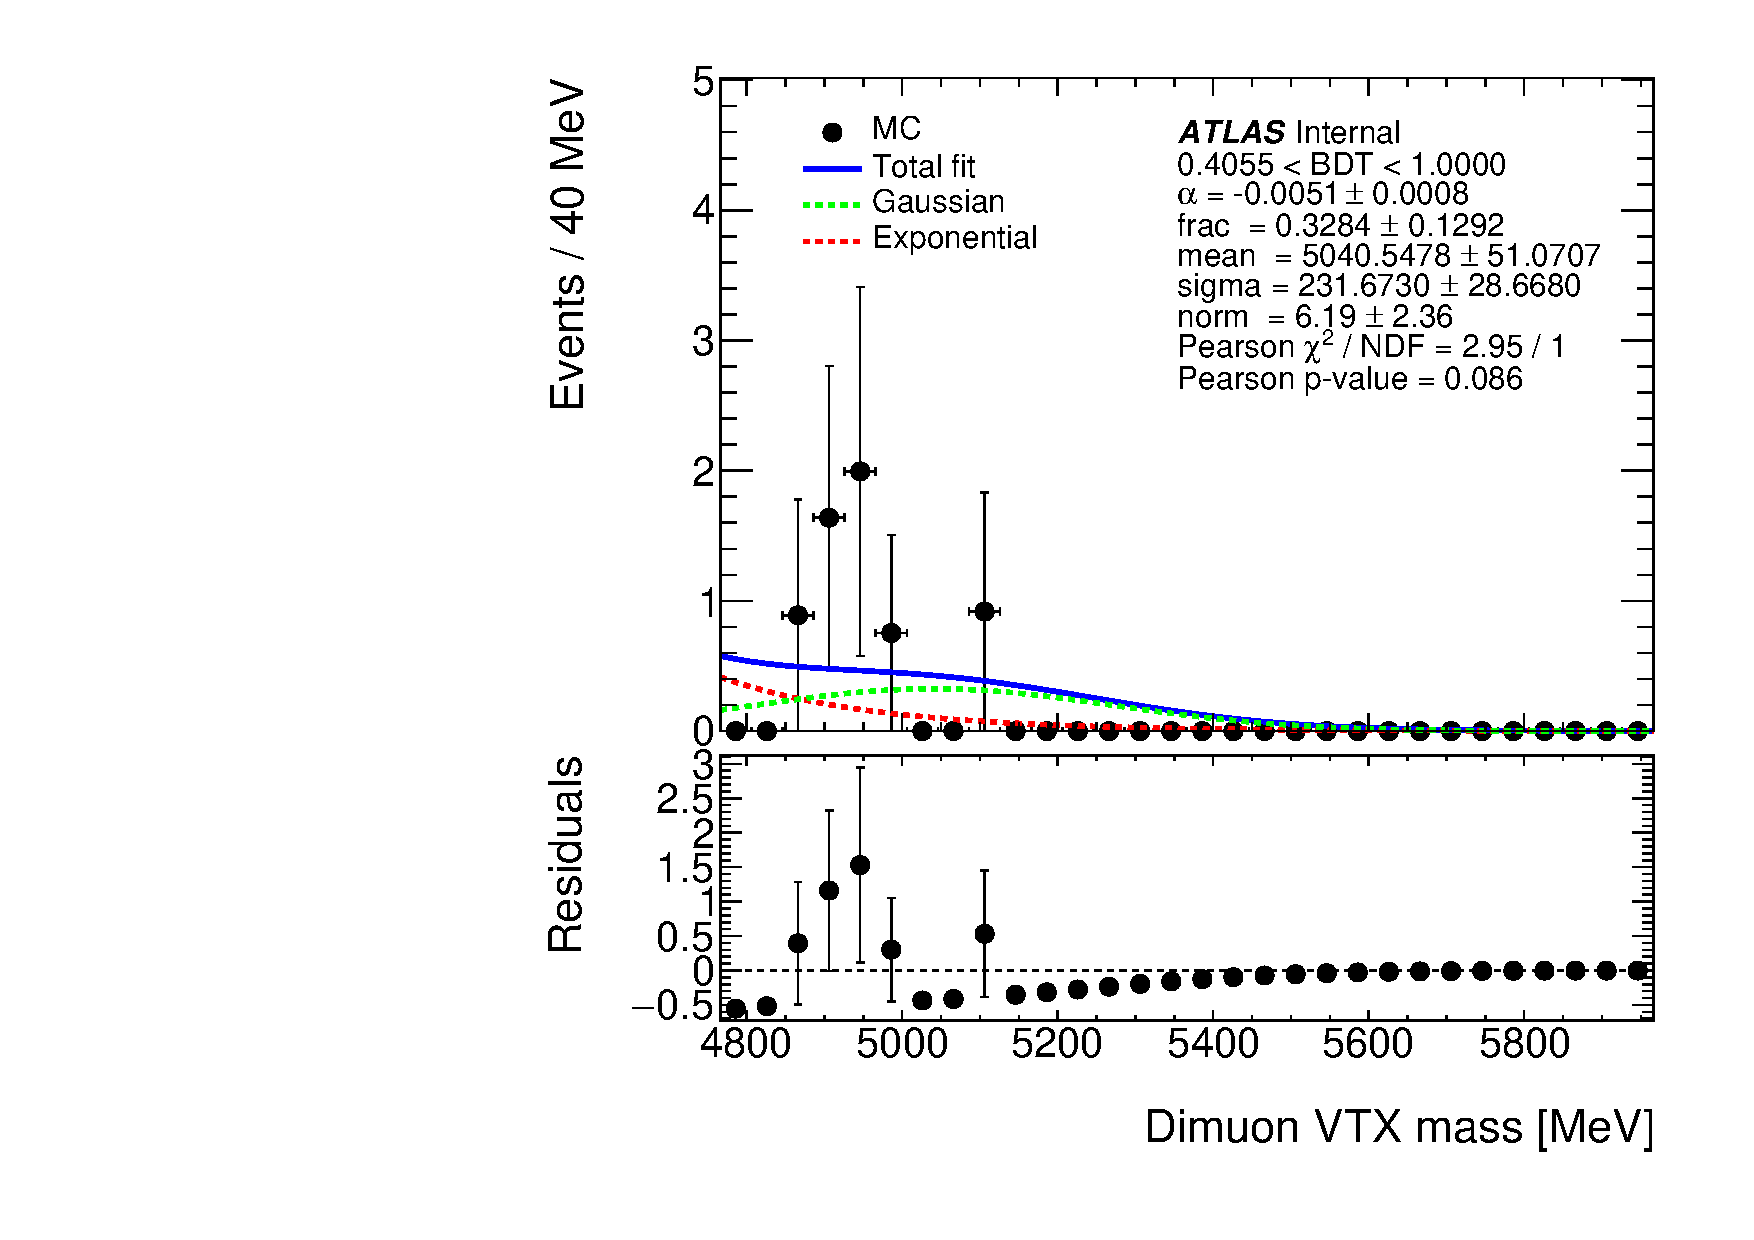
\includegraphics[width=0.5\textwidth]{figures/SignalExtraction/out_fit_test_semilep_v2p4_loose_params_fixed_can_bin_3.pdf}
    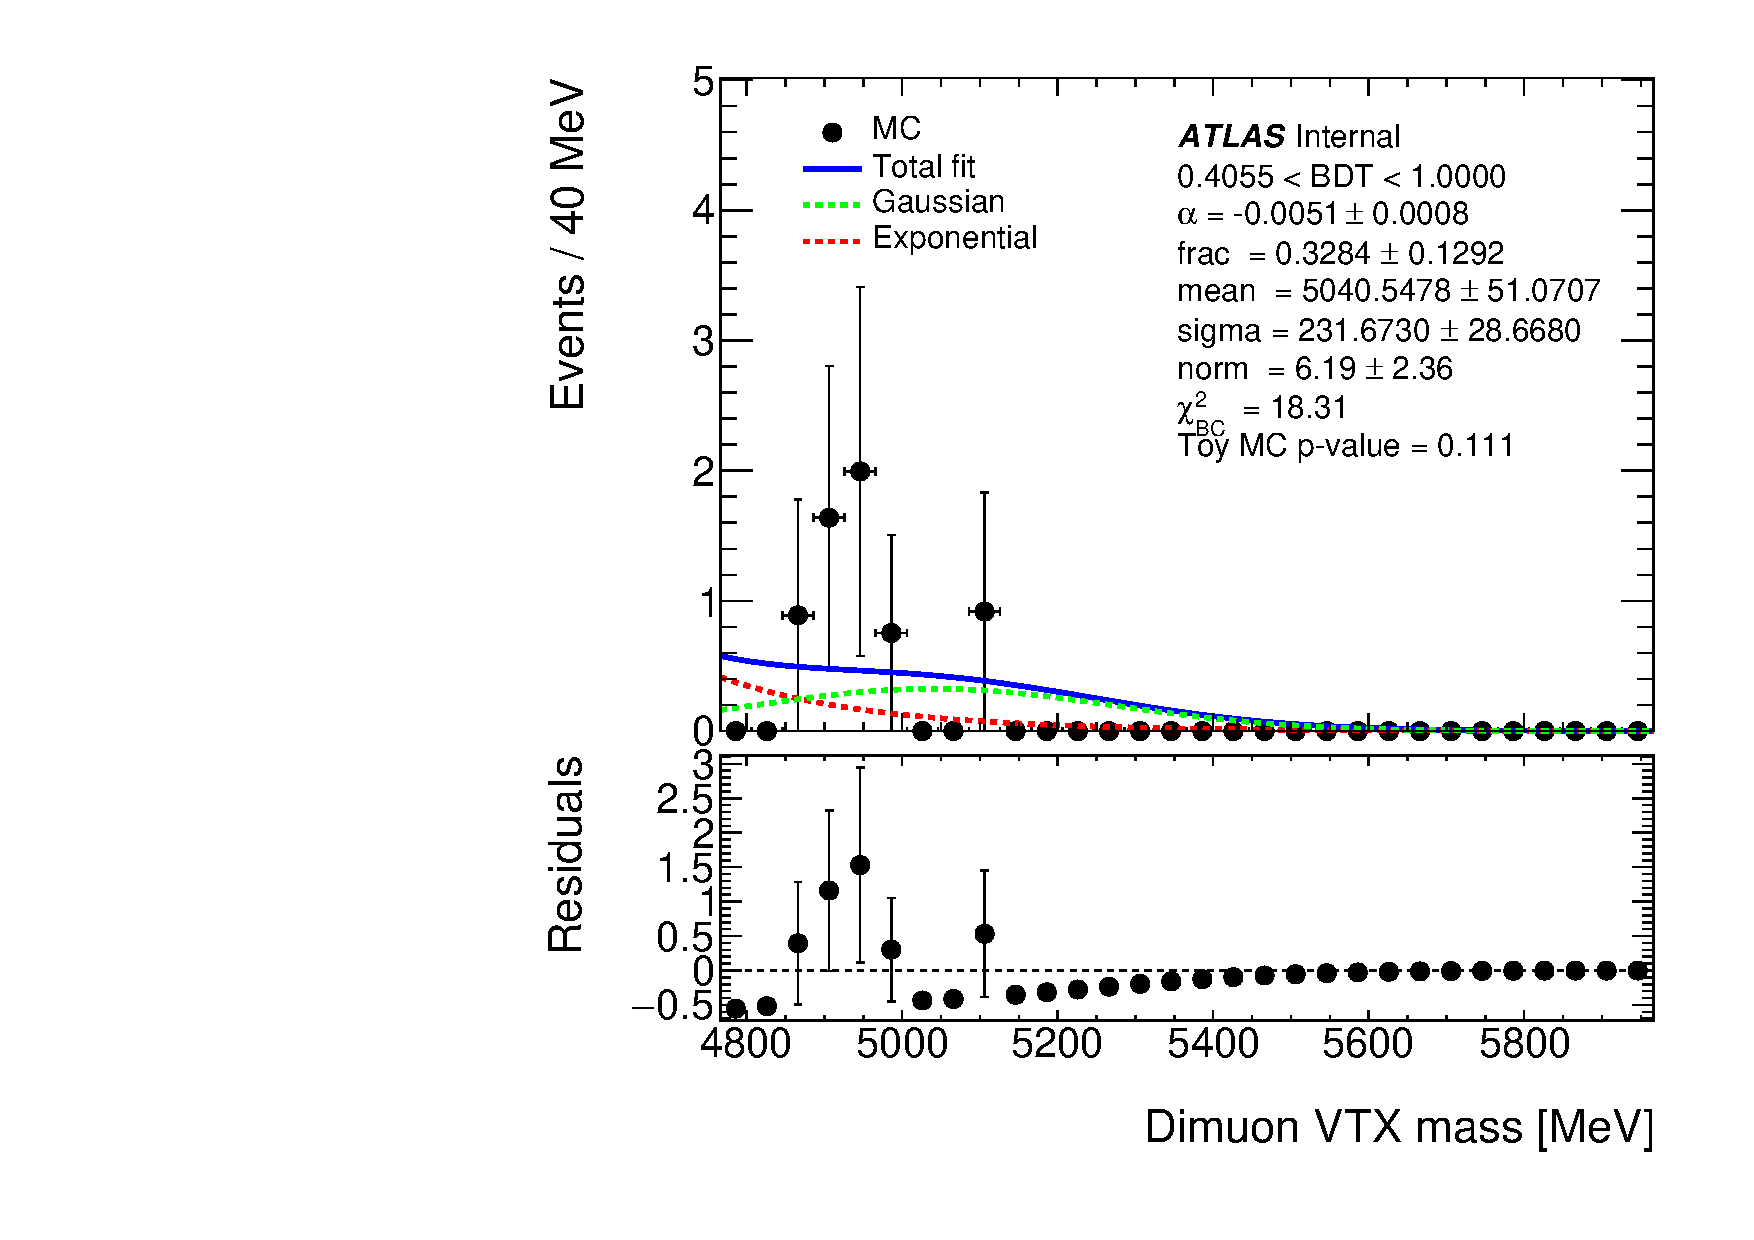
\includegraphics[width=0.5\textwidth]{figures/SignalExtraction/out_fit_semilep_v2p4_loose_params_fixed_BC_toy_MC_p_val_can_bin_3.pdf} % using toy MC BC Chi2 and p-value
    \label{fig:semilepMCfitBin3}
  }
  \caption{Unbinned extended maximum likelihood fits performed independently in BDT bin 0 \protect\subref{fig:semilepMCfitLooseBin0}, 1 \protect\subref{fig:semilepMCfitLooseBin1}, 2 \protect\subref{fig:semilepMCfitLooseBin2}, and 3 \protect\subref{fig:semilepMCfitLooseBin3} on the merged \BdPiMuNu, \BsKMuNu, \LPMuNu, and \LPMuNu exclusive MC samples. Applied to the merged MC sample are the final selections including requirements to pass the online trigger (and matching) but with only one muon passing the truth cuts. The shape parameters are fixed to the result of the fit in Figure~\ref{fig:semilepMCfitLoose}. Also shown are the fixed shape parameters, as well as the Baker-Cousins $\chi^{2}$, along with the p-value obtained by the frequentist toy MC approach discussed in section~\ref{subsubsec:BhhDataFits}.} 
  \label{fig:semilepMCfit}
\end{figure}

\clearpage